% Graphic for TeX using PGF
% Title: /home/andre/GIT Repos/AHCampher_thesis/diagrams/dmcplusramprate.dia
% Creator: Dia v0.97.1
% CreationDate: Thu Jan  6 16:23:31 2011
% For: andre
% \usepackage{tikz}
% The following commands are not supported in PSTricks at present
% We define them conditionally, so when they are implemented,
% this pgf file will use them.
\ifx\du\undefined
  \newlength{\du}
\fi
\setlength{\du}{15\unitlength}
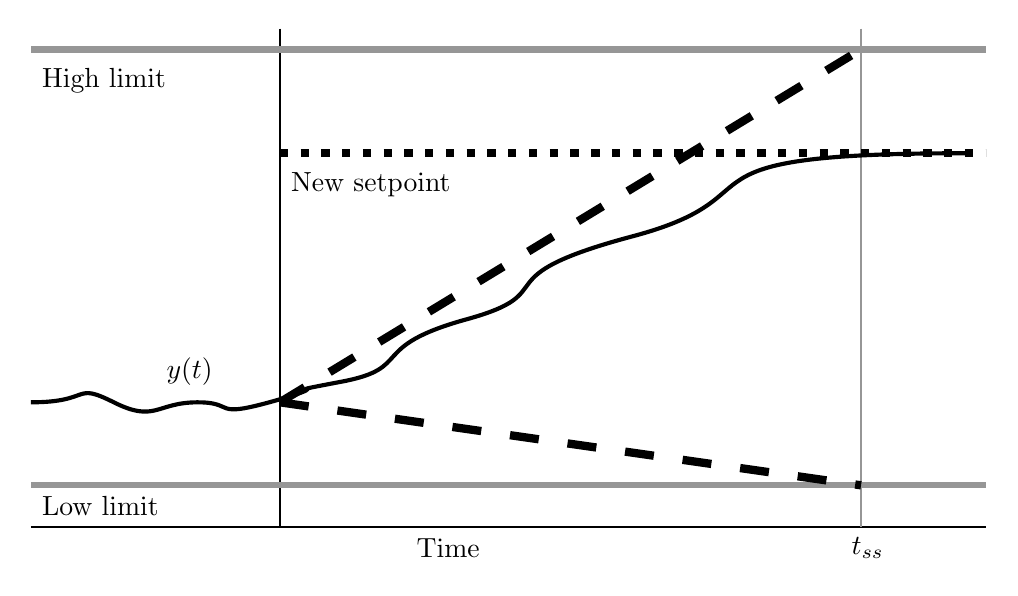
\begin{tikzpicture}
\pgftransformxscale{1.000000}
\pgftransformyscale{-1.000000}
\definecolor{dialinecolor}{rgb}{0.000000, 0.000000, 0.000000}
\pgfsetstrokecolor{dialinecolor}
\definecolor{dialinecolor}{rgb}{1.000000, 1.000000, 1.000000}
\pgfsetfillcolor{dialinecolor}
\pgfsetlinewidth{0.050000\du}
\pgfsetdash{}{0pt}
\pgfsetdash{}{0pt}
\pgfsetbuttcap
{
\definecolor{dialinecolor}{rgb}{0.000000, 0.000000, 0.000000}
\pgfsetfillcolor{dialinecolor}
% was here!!!
\definecolor{dialinecolor}{rgb}{0.000000, 0.000000, 0.000000}
\pgfsetstrokecolor{dialinecolor}
\draw (10.000000\du,15.000000\du)--(33.000000\du,15.000000\du);
}
\pgfsetlinewidth{0.050000\du}
\pgfsetdash{}{0pt}
\pgfsetdash{}{0pt}
\pgfsetbuttcap
{
\definecolor{dialinecolor}{rgb}{0.000000, 0.000000, 0.000000}
\pgfsetfillcolor{dialinecolor}
% was here!!!
\definecolor{dialinecolor}{rgb}{0.000000, 0.000000, 0.000000}
\pgfsetstrokecolor{dialinecolor}
\draw (16.000000\du,3.000000\du)--(16.000000\du,15.000000\du);
}
\pgfsetlinewidth{0.150000\du}
\pgfsetdash{}{0pt}
\pgfsetdash{}{0pt}
\pgfsetbuttcap
{
\definecolor{dialinecolor}{rgb}{0.588235, 0.588235, 0.588235}
\pgfsetfillcolor{dialinecolor}
% was here!!!
\definecolor{dialinecolor}{rgb}{0.588235, 0.588235, 0.588235}
\pgfsetstrokecolor{dialinecolor}
\draw (33.000000\du,3.500000\du)--(10.000000\du,3.500000\du);
}
\pgfsetlinewidth{0.150000\du}
\pgfsetdash{}{0pt}
\pgfsetdash{}{0pt}
\pgfsetbuttcap
{
\definecolor{dialinecolor}{rgb}{0.588235, 0.588235, 0.588235}
\pgfsetfillcolor{dialinecolor}
% was here!!!
\definecolor{dialinecolor}{rgb}{0.588235, 0.588235, 0.588235}
\pgfsetstrokecolor{dialinecolor}
\draw (33.000000\du,14.000000\du)--(10.000000\du,14.000000\du);
}
% setfont left to latex
\definecolor{dialinecolor}{rgb}{0.000000, 0.000000, 0.000000}
\pgfsetstrokecolor{dialinecolor}
\node[anchor=west] at (19.000000\du,15.500000\du){Time};
\pgfsetlinewidth{0.050000\du}
\pgfsetdash{}{0pt}
\pgfsetdash{}{0pt}
\pgfsetbuttcap
{
\definecolor{dialinecolor}{rgb}{0.588235, 0.588235, 0.588235}
\pgfsetfillcolor{dialinecolor}
% was here!!!
\definecolor{dialinecolor}{rgb}{0.588235, 0.588235, 0.588235}
\pgfsetstrokecolor{dialinecolor}
\draw (30.000000\du,3.000000\du)--(30.000000\du,15.000000\du);
}
\pgfsetlinewidth{0.200000\du}
\pgfsetdash{{\pgflinewidth}{0.040000\du}}{0cm}
\pgfsetdash{{\pgflinewidth}{0.300000\du}}{0cm}
\pgfsetbuttcap
{
\definecolor{dialinecolor}{rgb}{0.000000, 0.000000, 0.000000}
\pgfsetfillcolor{dialinecolor}
% was here!!!
\definecolor{dialinecolor}{rgb}{0.000000, 0.000000, 0.000000}
\pgfsetstrokecolor{dialinecolor}
\draw (16.000000\du,6.000000\du)--(33.000000\du,6.000000\du);
}
\pgfsetlinewidth{0.200000\du}
\pgfsetdash{{1.500000\du}{1.500000\du}}{0\du}
\pgfsetdash{{0.700000\du}{0.700000\du}}{0\du}
\pgfsetbuttcap
{
\definecolor{dialinecolor}{rgb}{0.000000, 0.000000, 0.000000}
\pgfsetfillcolor{dialinecolor}
% was here!!!
\definecolor{dialinecolor}{rgb}{0.000000, 0.000000, 0.000000}
\pgfsetstrokecolor{dialinecolor}
\draw (16.000000\du,12.000000\du)--(30.000000\du,3.500000\du);
}
\pgfsetlinewidth{0.200000\du}
\pgfsetdash{{0.700000\du}{0.700000\du}}{0\du}
\pgfsetdash{{0.700000\du}{0.700000\du}}{0\du}
\pgfsetbuttcap
{
\definecolor{dialinecolor}{rgb}{0.000000, 0.000000, 0.000000}
\pgfsetfillcolor{dialinecolor}
% was here!!!
\definecolor{dialinecolor}{rgb}{0.000000, 0.000000, 0.000000}
\pgfsetstrokecolor{dialinecolor}
\draw (16.000000\du,12.000000\du)--(30.000000\du,14.000000\du);
}
\pgfsetlinewidth{0.100000\du}
\pgfsetdash{}{0pt}
\pgfsetdash{}{0pt}
\pgfsetmiterjoin
\pgfsetbuttcap
{
\definecolor{dialinecolor}{rgb}{0.000000, 0.000000, 0.000000}
\pgfsetfillcolor{dialinecolor}
% was here!!!
\definecolor{dialinecolor}{rgb}{0.000000, 0.000000, 0.000000}
\pgfsetstrokecolor{dialinecolor}
\pgfpathmoveto{\pgfpoint{10.000000\du}{12.000000\du}}
\pgfpathcurveto{\pgfpoint{11.500000\du}{12.000000\du}}{\pgfpoint{11.000000\du}{11.500000\du}}{\pgfpoint{12.000000\du}{12.000000\du}}
\pgfpathcurveto{\pgfpoint{13.000000\du}{12.500000\du}}{\pgfpoint{13.016650\du}{12.007292\du}}{\pgfpoint{14.000000\du}{12.000000\du}}
\pgfpathcurveto{\pgfpoint{14.983350\du}{11.992708\du}}{\pgfpoint{14.300200\du}{12.412500\du}}{\pgfpoint{15.900100\du}{11.956250\du}}
\pgfpathcurveto{\pgfpoint{17.500000\du}{11.500000\du}}{\pgfpoint{15.750000\du}{11.833333\du}}{\pgfpoint{17.500000\du}{11.500000\du}}
\pgfpathcurveto{\pgfpoint{19.250000\du}{11.166667\du}}{\pgfpoint{18.083333\du}{10.666667\du}}{\pgfpoint{20.500000\du}{10.000000\du}}
\pgfpathcurveto{\pgfpoint{22.916667\du}{9.333333\du}}{\pgfpoint{20.750000\du}{9.000000\du}}{\pgfpoint{24.500000\du}{8.000000\du}}
\pgfpathcurveto{\pgfpoint{28.250000\du}{7.000000\du}}{\pgfpoint{25.030000\du}{6.000000\du}}{\pgfpoint{32.500000\du}{6.000000\du}}
\pgfusepath{stroke}
}
% setfont left to latex
\definecolor{dialinecolor}{rgb}{0.000000, 0.000000, 0.000000}
\pgfsetstrokecolor{dialinecolor}
\node[anchor=west] at (13.000000\du,11.2500000\du){$y(t)$};
% setfont left to latex
\definecolor{dialinecolor}{rgb}{0.000000, 0.000000, 0.000000}
\pgfsetstrokecolor{dialinecolor}
\node[anchor=west] at (10.000000\du,4.25000000\du){High limit};
% setfont left to latex
\definecolor{dialinecolor}{rgb}{0.000000, 0.000000, 0.000000}
\pgfsetstrokecolor{dialinecolor}
\node[anchor=west] at (10.000000\du,14.500000\du){Low limit};
% setfont left to latex
\definecolor{dialinecolor}{rgb}{0.000000, 0.000000, 0.000000}
\pgfsetstrokecolor{dialinecolor}
\node[anchor=west] at (16.000000\du,6.7500000\du){New setpoint};
% setfont left to latex
\definecolor{dialinecolor}{rgb}{0.000000, 0.000000, 0.000000}
\pgfsetstrokecolor{dialinecolor}
\node[anchor=west] at (29.500000\du,15.500000\du){$t_{ss}$};
\end{tikzpicture}
